% This is LLNCS.DEM the demonstration file of
% the LaTeX macro package from Springer-Verlag
% for Lecture Notes in Computer Science,
% version 2.3 for LaTeX2e
%
\documentclass{llncs}
%
\usepackage{makeidx} % allows for indexgeneration
\usepackage{graphicx}
\usepackage{multicol}
\usepackage{subfigure}
\usepackage{mathptmx} % use Times fonts if available on your TeX system
\usepackage{setspace}
%
\begin{document}
\title{Robotic Validation of an Inter-disciplinary Generic\\
Model of Self-regulated Division of Labour\\ in Social Systems
\thanks{This research has been funded by the Engineering and Physical Sciences Research Council (EPSRC), UK, grant reference EP/E061915/1.}
}
%\subtitle{Do you have a subtitle?\\ If so, write it here}
\titlerunning{Robotic Validation of an Inter-disciplinary Generic Model\\
of Self-regulated Division of Labour in Social Systems } % if too long for running head
\author{Md Omar Faruque Sarker \and
Torbjorn Dahl %etc.
}
%\authorrunning{Short form of author list} % if too long for running head
\institute{
Robotic Intelligence Lab,
Newport Business School\\
University of Wales, Newport,
Allt-yr-yn Campus\\ Allt-yr-yn Avenue, Newport, NP205XR, UK\\
\email{Mdomarfaruque.Sarker@newport.ac.uk\\
Torbjorn.Dahl@newport.ac.uk}
}
%\date{Received: / / Accepted: / / }
% The correct dates will be entered by the editor
\maketitle
\begin{abstract}
Multi-agent task allocation or division of labour (DoL) is a challenging research issue in the field of multi-agent and multi-robot systems. Unlike the swarm robotic approach, which is inspired by biological systems alone and commonly aims for minimal intelligence agents, we propose to solve DoL in multi-robots based on a set of observed generic rules of DoL from biological and human social systems. These bottom-up rules describe the phenomena of self-regulated DoL in terms of attractive fields between robots and tasks. The concrete form of these rules, termed as \textit{attractive filed model} (AFM), offers a scalable solution to the above DoL problem. Unlike having strong dependence to local interactions by most of the existing approaches, our model states that self-regulatory DoL can be established by AFM without maintaining a strong form of local interactions. Our approach has been validated by experiments with 16 physical E-puck robots in an area of about 4$m^2$.
%\keywords{First keyword \and Second keyword \and More}
%% \PACS{PACS code1 \and PACS code2 \and more}
%% \subclass{MSC code1 \and MSC code2 \and more}
\end{abstract}
%\addtolength{\parskip}{-3.5mm}
\section{Introduction}
\label{sec:intro}
%\vspace{2mm}
Scientific studies show that a large number of animal as well as human social systems grow, evolve and generally continue functioning well by the virtue of their individual self-regulatory mechanism of division of labour (DoL) \cite{Camazine+2001}. It is interesting to note that in animal societies this has been accomplished years after years without a central authority or an explicit planning and coordinating element. Indirect communication such as stigmergy is rather used to exchange information among individuals \cite{Bonabeau+1999}. 
In MRS domain, \textit{multi-robot task allocation} (MRTA) is a common research challenge \cite{Gerkey+2004}. In case of a real-world dynamic environment, it is generally identified as the question of assigning tasks in an appropriate time to the appropriate robots considering the changes of the environment and/or the performance of other team members . This is an optimal assignment problem also known as NP-hard, where optimal solutions can not be found quickly for large problems \cite{Parker2008}. The reason of such complexities lies on the fact that there is no central planner or coordinator for task assignments and the capabilities of robots are limited to sense, to communicate and to interact locally \cite{Lerman+2006}. None of them has the complete knowledge of the past, present or future actions of other robots as well as they don't have the complete view of the world state. For a larger team of robots (more than 10 robots) the bandwidth of local communication channel is also limited. In practical implementations the computational and communication bandwidth requirements restrict the solution quality of the problem \cite{Gerkey+2004,Lerman+2006}.\\
Traditionally task allocation in a multi-agent system is divided into two major categories: 1) Predefined (off-line) and 2) Emergent (real-time) task-allocation \cite{Shen+2001}. Usually predefined task allocation method uses either centralized coordination or distributed task-allocation approach. Distributed task-allocation approach is again subdivided into three subcategories, namely 1) direct allocation, 2) task allocation by delegation and 3) task allocation through bidding.
In MRS domain, early research on predefined task-allocation approach has been dominated mainly by intentional coordination, use of dynamic role assignment \cite{Parker2008} and market-based bidding approach \cite{Dias+2006}. In intentional approach robots uses direct task-allocation method to communicate and to negotiate for assigning tasks. This is preferred approach among MRS research community since it is easily understood, easier to design, implement and analyse formally. However this approach usually works well only when the MRS team-size is small ($ \leq $ 10 robots) \cite{Lerman+2006}. When the number of robots  increases, their computational requirements and interaction complexities increase significantly that reduce their shared communication bandwidth and as a result, these make the overall team performance poor. Thus this approach fails to scale well when the number of tasks and robots are increased.\\ 
On the other hand emergent task-allocation approach relies on the emergent group behaviours, such as emergent cooperation \cite{Lerman+2006}, adaptation rules \cite{Liu+2007} etc., that lead to task allocation with local sensing, local interactions and typically little or no explicit communication or negotiations between robots. They are more scalable to large team size and more robust via parallelism and redundancy. However these systems are not free from drawbacks. Most of researchers complain that they are difficult to design, analyse formally and implement practically \cite{Gerkey+2004,Lerman+2006}. The MRTA solutions from these systems are also sub-optimal. Since the emergence is a result of interactions among robots and their environment, in such systems it is also difficult to predict exact behaviours of robots and overall system performance.\\
The existing challenges of emergent task allocation approaches leads us to investigate for a suitable alternative. From the technological advances in electronics and communication, it is clear to us that the size of MRS as well as the task complexities will ever grow faster and scalability and performance will remain as major issues of MRS research. If we look at nature we can find that task allocation in animal or insect societies is governed by non-centralized rules and they are much more self-regulated and self-stabilized \cite{Camazine+2001,Bonabeau+1999}. Moreover from our study of sociology \cite{Sayer+1992}, cybernetics \cite{Beer1981}, strategic management  \cite{Kogut2000}) and related other disciplines we can find that decentralized self-regulated systems exist and they can grow and achieve viability over time. From the multi-disciplinary studies of these complex systems we believe that a set of generic rules can be derived for the emergence of division of labour in MRS. Primarily these rules should deal with the issue of deriving local control laws for facilitating the emergence of global team behaviour \cite{Parker2008}.\\
As a part of a collaborative project, we have studied social systems in ants, humans and robots and have developed a common formal model of division of labour that is used to analyse systems from the three disciplines involved \cite{Elsa}. In this paper, we have presented this model in a robotic social system's context. Section 2 describes our model of self-regulated DoL and an associated model of communication for different entities of our system. Section 3 introduces our experiment set-up and interaction among hardware, software  and communication modules. Section 4 presents our experiment design with a set of parameters and observables. Section 5 discusses our experimental results. Section 6 concludes this paper.
%
%%%%%%%%%%%%%%%%%%%%%%%%%%%%%%%%%%%%%%%%%%%%%%%%%%%%%%%%%%%%%%%%%%%%%%%%%%%%%%%%%%%%
%\addtolength{\topskip}{-15mm}
\section{Modeling}
\label{sec:model}
\subsection{Model for Self-Regulatory DoL}
Our model of self-regulated DoL is based on AFM. It provides us a generic framework for implementing self-regulatory DoL in robots. Here we briefly describe how this model gives our robots self-regulatory DoL behaviours, particularly task-specialization, concurrency, flexibility and robustness.
%%
\begin{figure}
\begin{minipage}[t]{0.48\linewidth}
\centering
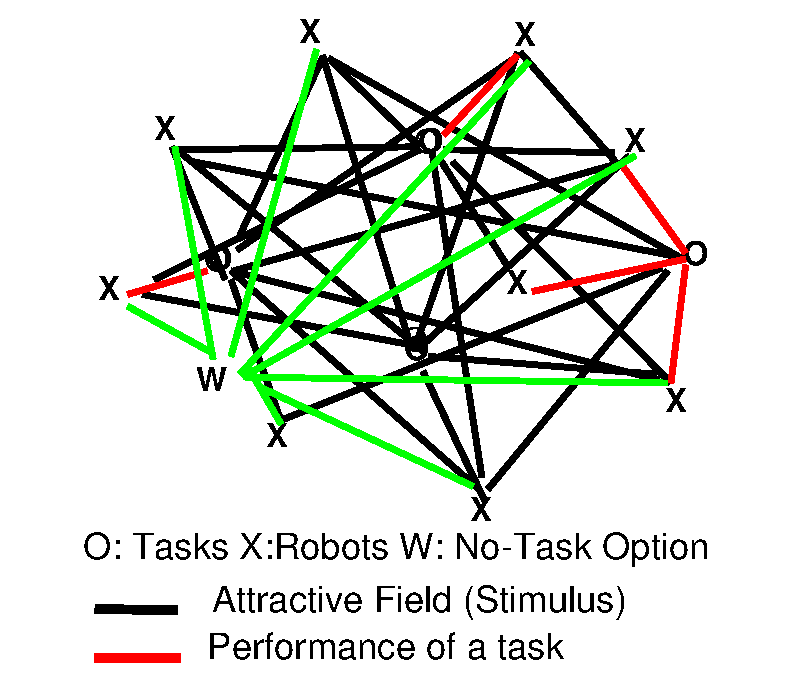
\includegraphics[height=5cm, angle=0]
{../dia-files/AFM-Diag2.eps}
%figure caption is below the figure
\caption{\small Atrractive Filed Model}
\label{fig:afm} % Give a unique label
\end{minipage}
\hspace{0.5cm}
\begin{minipage}[t]{0.48\linewidth}
\centering
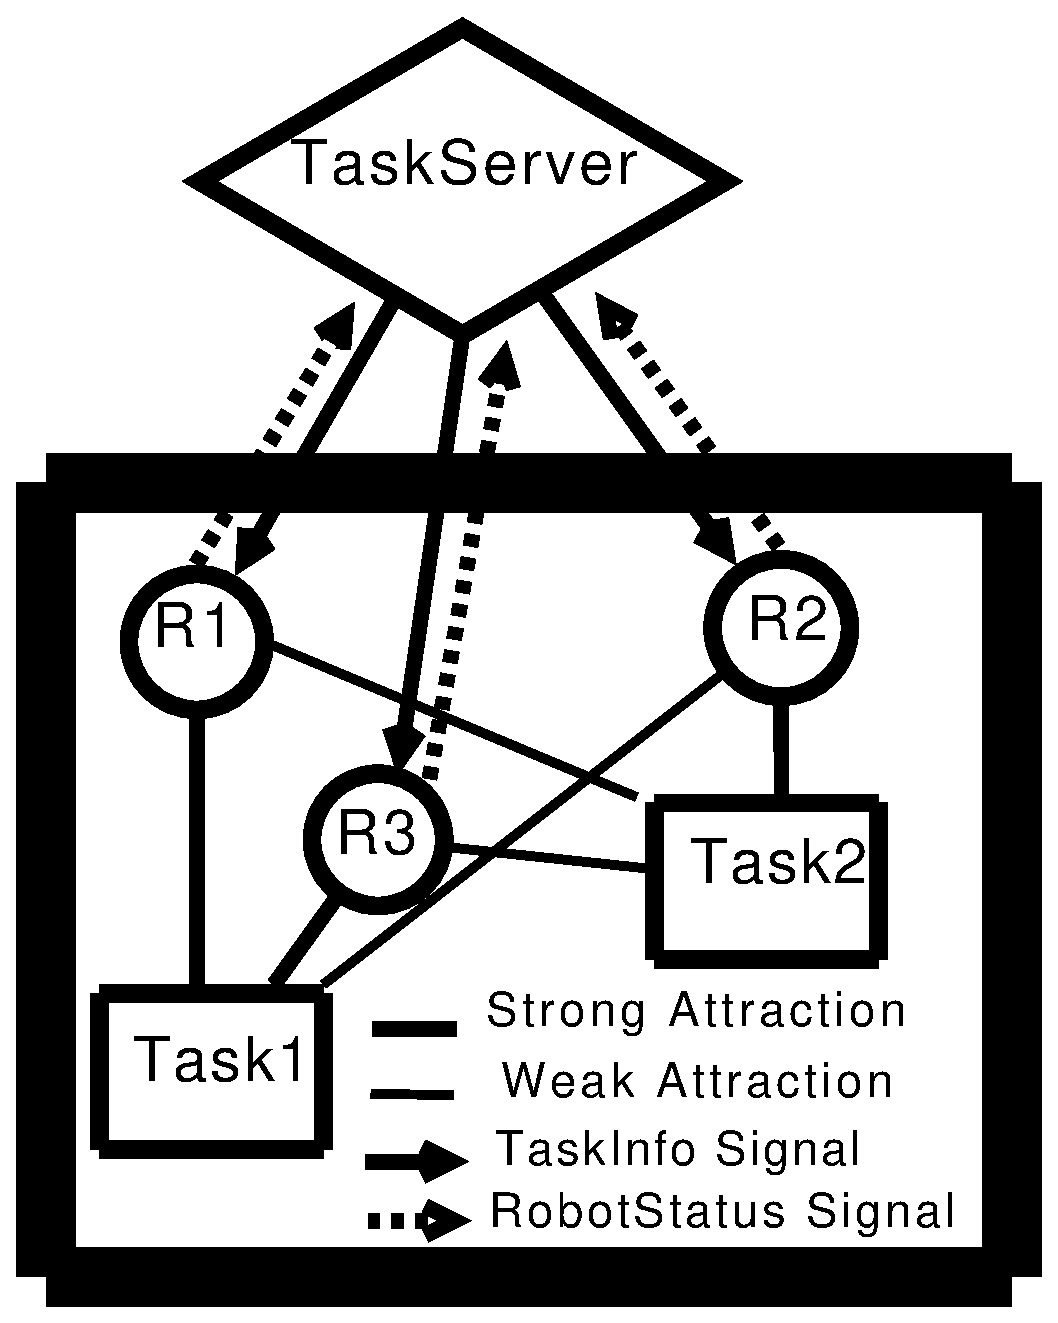
\includegraphics[height=5cm, angle=0]{../dia-files/CentralizedComm.eps}
\caption{\small Centralized Communication Model}
\label{fig:ccm} % Give a unique label
\end{minipage}
\end{figure}
%%
Let us consider a manufacturing shop floor scenario where N number of mobile robots are required to attend to M number of shop tasks spread over a fixed area A. Let these tasks be represented by a set of small rectangular boxes resembling to manufacturing machines. Let $R_1$, $R_2$ … $R_n$ be the set of all robots and $J_1$, $J_2$ … $J_m$ be the set of all tasks. Each task $j$ has an associated task-urgency $\phi_j$ that indicates its relative importance over time. If a robot attends to a task $j$ in x$^{th}$ time-step, value of $\phi_j$ will decreases by a small amount $\delta_\phi$ in (x+1)$^{th}$ time-step. On the other hand, if a task has not been served by any robot in x$^{th}$ time-step, $\phi_j$ will increase by another small amount in (x+1)$^{th}$ time-step. In order to complete a shop task $J_1$, a robot $R_1$ needs to reach within a fixed boundary $D_{j1}$ of $J_1$. If a robot completes a task $j$ we say that it learns about it and this will increase this robot's likelihood of selecting that task in next step. We call this variable affinity of a robot to that task as its sensitization $k_j$ . If a robot does not do a task $j$ for some time, we say that it forgets about $j$ and $k_j$ has been decreased.\\
According AFM, all robots will establish attractive fields to all tasks due to the presence of a system-wide continuous flow of information. The strength of these attractive fields called stimulus will vary according to the distances between robots and tasks, task-urgencies and corresponding sensitizations of robots. This is encoded in Eq. \ref{eqn1}.
%\addtolength{\abovedisplayskip}{-15mm}
\begin{small}
\begin{multicols}{2}
\begin{equation}
S_{j}^{i} = tanh\{\frac{k_{j}^{i}}{d+\delta } \phi _{j}\}
\label{eqn1}
\end{equation}
\vspace*{0.25cm}
\begin{equation}
P_{j}^{i} = \frac{S_{j}^{i}}{\sum_{j}^{}S_{j}^{i}}
\label{eqn2}
\end{equation}
\end{multicols}
\end{small}
%\addtolength{\belowdisplayskip}{-1mm}
%\vspace{2mm}
Eq. \ref{eqn1} says that the stimuli of a robot $i$ to a particular task $j$, $S_{j}^{i}$ depends on $i$'s spatial distance $d_{ij}$ to $j$, level of sensitization to $j$, $k_{j}^{i}$) and perceived urgency of that task ($\phi _{j}$). We use a vary small value $\delta$ in Eq. \ref{eqn1} to prevent division by zero. The probability of selecting each task has been determined by a probabilistic method outlined in Eq. \ref{eqn2}.
AFM suggests concurrency of a self-regulatory system by specifying at least two task options: 1) doing a task and 2) not doing a task. In robots, the latter can be be treated as random walking. So in any time-step a robot will choose from M+1 tasks. Let $T_a$ be the allocated time to accomplish a task. If $R_1$ can enter inside the task boundary within $T_a$ time it waits there until $T_a$ elapsed. Otherwise it will select a different task.
\subsection{Model of Communication}
In order to establish a system-wide continuous flow of information, we need to implement a suitable communication system for our robots. Here we have presented a centralized model of communication for our manufacturing shop-floor scenario.
%% 
As shown in Fig. \ref{fig:ccm}, in this model there exists a centralized \textit{
TaskServer} that is responsible for disseminating task information to robots. The content of task information can be physical location of task in the environment, urgency and so on. TaskServer delivers this information by emitting \textit{TaskInfo} signals periodically. The method of signal emission depends on a particular communication technology. For example, in a wireless network it can be a message broadcast.
Task-Server has another interface for catching feedback signals from robots. The \textit{RobotStatus} signal can be used to inform TaskServer about a robot's current task id, its device status and so on. TaskServer uses this information to update relevant part of task information such as, task-urgency. This up-to-date information is sent in next TaskInfo signal.\\
In Fig. \ref{fig:ccm} an initial configuration of this model has been presented. Upon receiving an initial TaskInfo signal robot $R_1$  has shown strong attraction towards $Task1$ and robot $R_3$ has shown strong attraction toward $Task2$. This can be inferred from Eq. \ref{eqn1} that says if the initial task urgencies and sensitizations for all tasks are same, a robot will strongly be attracted towards a task that is relatively closer to it.
%%%%%%%%%%%%%%%%%%%%%%%%%%%%%%%%%%%%%%%%%%%%%%%%%%%%%%%%%%%%%%%%%%%%%%%%%%%%%%%%%%% 
\section{Implementation}
\label{sec:impl}
\begin{figure}
\centering
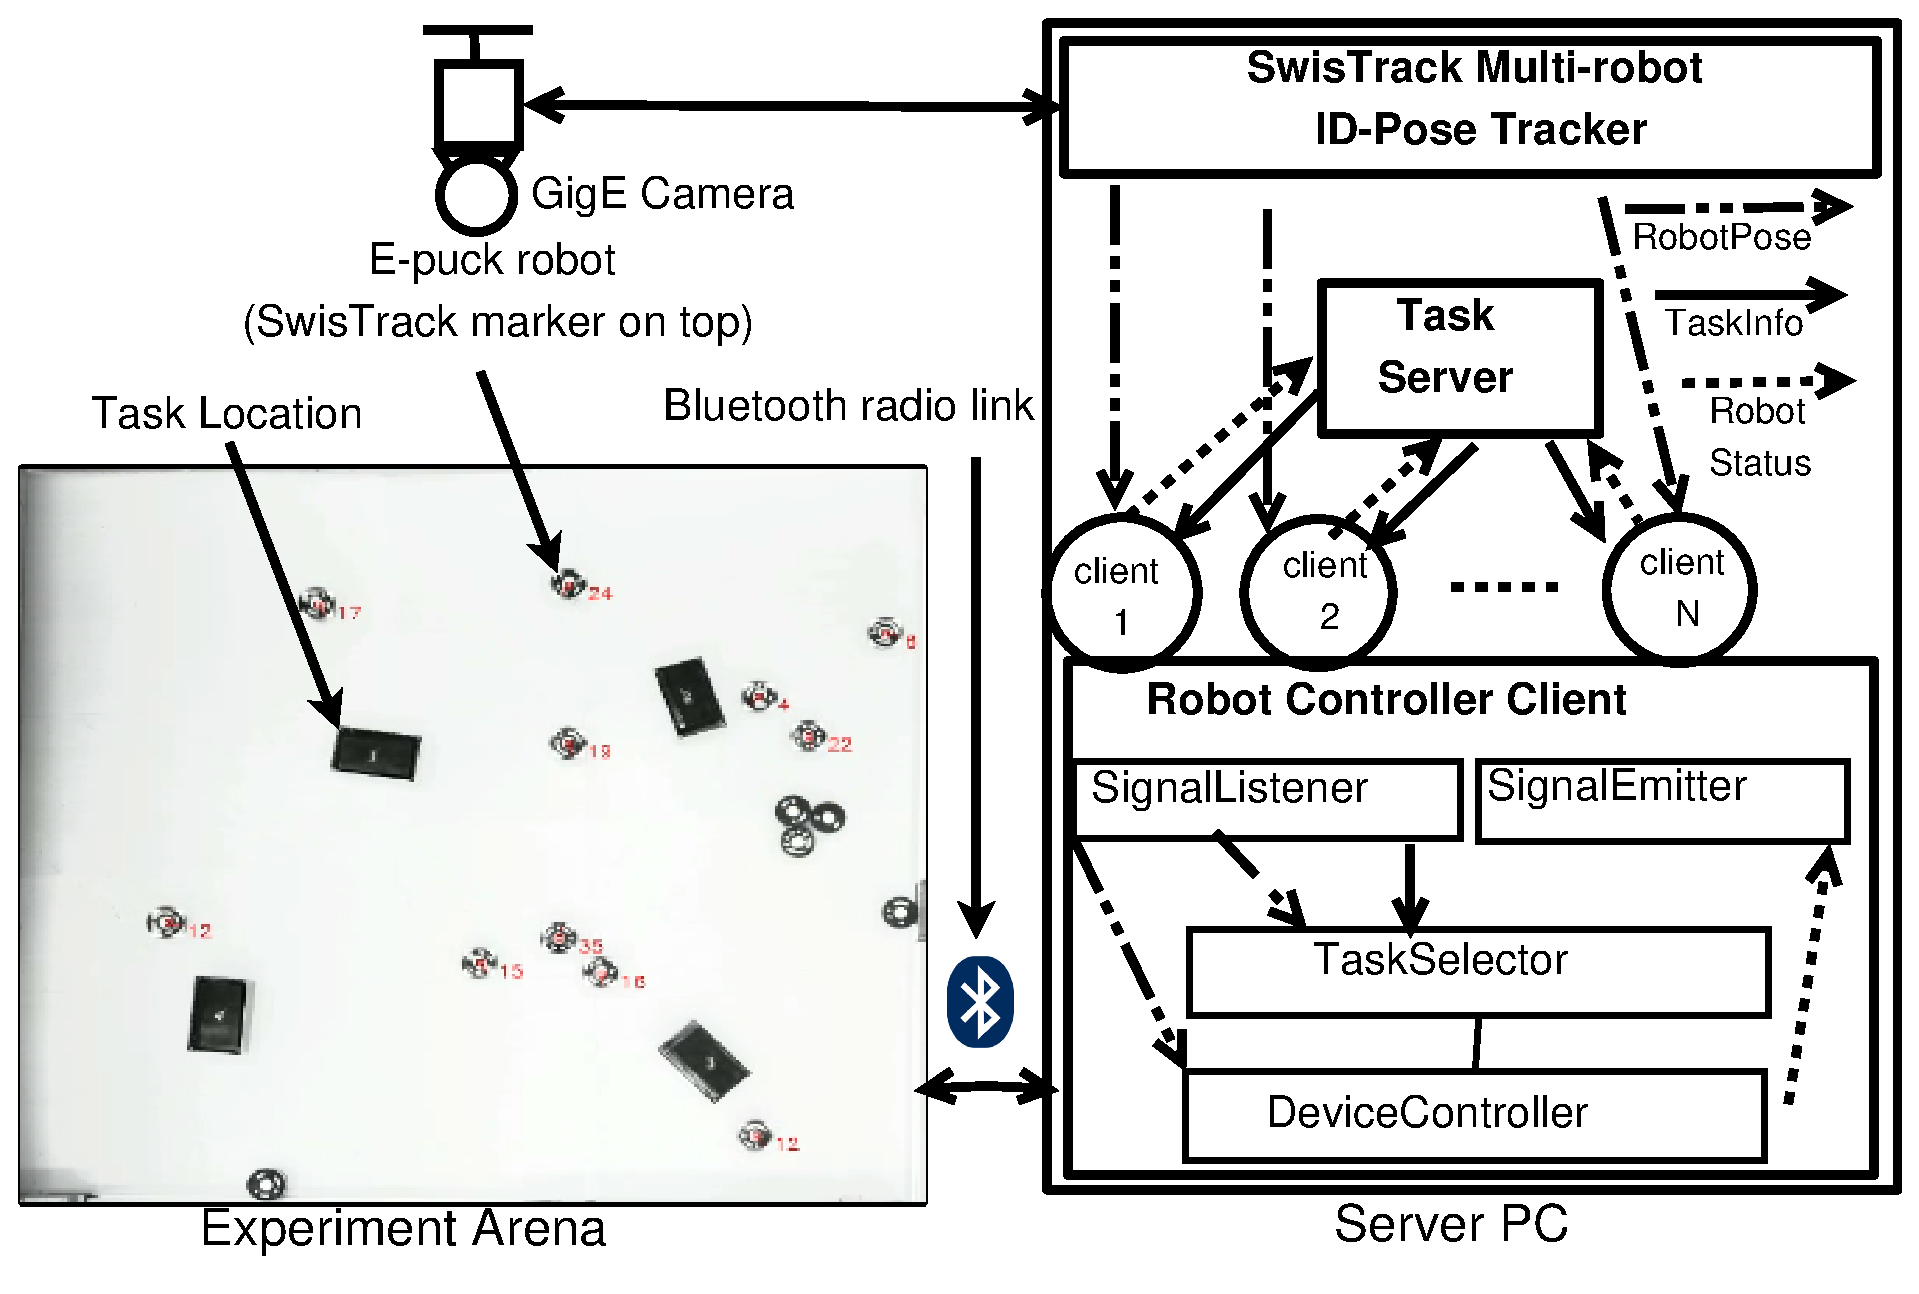
\includegraphics[height=7cm, angle=0]
{../dia-files/RIL-Expt-Setup1.eps}
%figure caption is below the figure
\caption{\small Hardware and software setup}
\label{fig:setup} % Give a unique label
\end{figure}
We have developed a system where up to 40 E-puck robots \cite{Epuck} can operate together according to the generic rules of the AFM. In order to track these robots we have used SwisTrack \cite{SwisTrack}, a state of the art open-source, multi-agent tracking system, along with a16-megapixel overhead GigE camera. This set-up gives us the position, heading and id of each of the robots at a frequency of 1. The interaction of the hardware and software of our system is illustrated in Fig. \ref{fig:setup}. \\
For inter-process communication (IPC), we have used D-Bus technology \cite{DBus}. We have developed an IPC component for SwisTrack (hereafter called as \textit{SwisTrack D-Bus Server}) that can broadcast id and pose of all robots in real-time over our server's D-Bus interface.\\
Apart from SwisTrack, we have implemented two major software modules: TaskServer and Robot-Controller-Client (RCC). They are developed in Python with its state of the art \textit{Multiprocessing} module \cite{Multiprocessing}. This python module simplifies our need to manage data sharing and synchronizing among different sub-processes. As shown in Fig. \ref{fig:setup}, RCC consists of four sub-processes: SignalListener, SignalEmitter, TaskSelector, DeviceController. SignalListener catches RobotPose and TaskInfo signals from SwisTrack D-Bus Server and Task-Server respectively. SignalEmitter emits RobotStatus signal for TaskServer. TaskSelector selects a particular task based on information obtained from TaskInfo and RobotPose signals. This selected task has been notified to DeviceController that actually moves a robot to a target task. DeviceController uses Bluetooth radio link as a communication medium between RCC and physical E-puck. Data sharing and synchronization among all four sub-processes are done using Data-manger and Event interfaces of Python Multiprocessing module. Similar to RCC, Task-Server also has three sub-processes: SignalListener, SignalEmitter and TaskInfoUpdater. SignalListener listens RobotInfo signal and passes corresponding info to TaskInfoUpdater that updates task urgency of all tasks based on AFM's guidelines. The updated information is then encoded as new TaskInfo signal and emitted by SignalEmitter. TaskInfo signal also contains location of all tasks that we have provided to TaskServer as start-up arguments.\\ 
To recap, our system works by repeating the following steps:
\begin{itemize}
\item SwisTrack grabs overhead camera image and finds id and pose of all robots. SwisTrack D-Bus Server periodically broadcast them as RobotPose D-Bus signal.
\item All RCC catch their individual RobotPose signal and a common TaskInfo signal from SwisTrack D-Bus Server and TaskServer respectively. They select a particular task or random walk based on AFM's guidelines. If a physical link between an E-puck robot and a RCC is established, this selected task is then started to execute. When a task-execution starts, each RCC emits its RobotStatus signal over D-Bus.
\item TaskServer updates task-urgencies after processing RobotStatus signal received from robots. This updated task-urgencies are then encoded in new TaskInfo signal and emitted by TaskServer in next step.
\end{itemize}
%%%%%%%%%%%%%%%%%%%%%%%%%%%%%%%%%%%%%%%%%%%%%%%%%%%%%%%%%%%%%%%%%%%%%%%%%%%%
\section{Experiment Design}
\label{sec:expt-design}
In order to validate AFM in robots we have designed a set of centralized communication experiments as outlined in \ref{sec:impl}. Here we describe our experimental parameters
and observables.
%
\begin{table}
\caption{Experimental parameters}
\label{table:params}
\begin{center}
\begin{tabular}{|l||c|}
\hline Parameter & Value\\
\hline Total number of robots ($N$) & 16\\
\hline Total number of tasks ($M$) & 4\\
\hline Experiment area ($A$) & 4 $m^2$\\
\hline Intial task urgency ($\Phi_{INIT}$) & 0.5\\
\hline Task urgency increase rate ($\Delta\phi_{INC}$) & 0.005\\
\hline Task urgency decrease rate ($\Delta\phi_{DEC}$) & 0.0025\\
\hline Intial sensitization ($K_{INIT}$) & 0.1\\
\hline Sensitization increase rate ($\Delta k_{INC}$) & 0.03\\
\hline Sensitization decrease rate ($\Delta k_{DEC}$) & 0.01\\
\hline A very small distance ($\delta$)& 0.000001\\
\hline Task info update interval ($\Delta TS_{u}$) & 5s\\
\hline Task info signal emission interval ($ \Delta TS_{e}$)& 2.5s\\
\hline Robot's task time-out interval ($\Delta RT_{to} $)& 10s\\
\hline
\end{tabular}
\end{center}
\end{table}
% 
\subsection{Parameters}
Table \ref{table:params} lists a set of essential parameters of our experiments. The following relationships are maintained for selecting task-urgency and sensitization parameters.
\begin{small}
\begin{equation}
\Delta\phi_{DEC} = \Delta\phi_{INC} \times \frac{N}{2 \times M}
\label{eqn:task-urgency}
\end{equation}
%
\begin{equation}
\Delta k_{DEC} = \frac{\Delta k_{INC}} {M - 1} 
\label{eqn:sensitization}
\end{equation}
\end{small}
%
\subsection{Observables}
We have defined a set of observables to benchmark our implementation. The first two observables, the changes in task-urgencies and the changes in robot sensitizations, give us an external and internal view of our system with respect to AFM respectively. Our third observable is to find changes in robot motions. This is completely objective measurement of our system. Our final measurement is the communication load which is specific to this particular implementation. They are briefly explained here.\\
\textbf{Changes in task-urgencies ($\Delta \Phi$): }
In our experiments, urgency of each task in each step has been logged. From the above design of task urgency, we can see that if a task is not served by any robot for 100 consecutive steps (500s), urgency of that task will reach from 0.5 to its maximum value 1.0. On the other hand, if a task is served by only one robot for 200 consecutive steps (1000s) urgency of that task will be 0. But in real experiment, it is more likely that more than one robot will serve a task. So urgency of a task will decrease $\Delta\phi_{DEC}$ times number of working robots on that task (based on AFM guidelines \cite{Elsa}). The overall changes in task urgencies will show the convergence behaviour of our system. A stable convergence will most likely map to a stable division of labour of the system.\\
\textbf{Changes in robot sensitizations ($\Delta K$): }
According AFM, as robots will do tasks they will specialize on each task by increasing or decreasing sensitizations (learning and forgetting). From our above design, we can see that if a robot starts doing a task with an initial sensitization of 0.1 and it repeatedly does it for 30 consecutive steps, we will be able to say that it has learnt it completely. On the other hand, with an initial sensitization of 0.1 if a robot does not do a task for 10 consecutive steps we will be able to say that it has forgotten that task completely.\\
\textbf{Changes in robot motions ($\Delta U$): }
As we might guess that initially the task urgencies will be relatively higher for all tasks so robots will need to do a lot of movements by switching from one tasks to another. But as the system convergences overall robot motions will be decreased. In order to observe this phenomenon we log the pose of robots in each time they receive pose signals.\\
\textbf{D-Bus Signals emitted by Task server ($S_f$):} 
In order to measure the communication load on our system and to benchmark Task server's D-Bus signalling performance we are also interested to log TaskInfo D-Bus signals. Since the emission of signals happens in a fixed time interval it is more likely that the overall communication load on the system will remain constant over time.
%
%%%%%%%%%%%%%%%%%%%%%%%%%%%%%%%%%%%%%%%%%%%%%%%%%%%%%%%%%%%
% 
\section{Results and Discussions}
\label{sec:results}
%%
In this section we have presented  our experimental results. We ran those experiments for about 40 minutes and averaged them from three iterations.
Fig. \ref{fig:raw-urgencies} shows the dynamic changes in task urgencies. Here we find that at about $100^{th}$ step all urgencies has stabilized near 0. The rise and fall of task urgencies show that our system is capable of providing a robust DoL. 
In order to describe our system's dynamic behaviour holistically we analyse the changes in task urgencies over time. Let $ \phi_{j, q}$ be the urgency of a task $j$ at $q^{th}$ step. In $(q+1)^{th}$ step, we can find the change of  urgency of task $j$ :\\
\begin{equation} 
\small
\delta \phi_{j, q+1} = ( \phi_{j, q+1} - \phi_{j, q}) 
\end{equation}
So we can calculate the sum of changes in urgencies of all tasks at $(q+1)^{th}$ step:
\begin{equation} 
\small
\Delta \Phi_{j, q+1} = \sum_{j=1}^{M} \delta \phi_{j, q+1} 
\label{eqn:Delta-Phi}
\end{equation}
Fig. \ref{fig:urgency-convergence} plots this sum of changes of task urgencies by a dashed line. If we consider the absolute change over a window $w$ of time in the following equation we can describe the overall changes of our systems in both positive and negative directions.
%
\begin{equation}
\small
\Delta \Phi_{jw, q+1} = \sum_{j=0}^{w-1} \left | \Delta \Phi_{q+j} \right |
\end{equation}
%
In order to find convergence in DoL we have calculated the sum of absolute changes in task urgencies over a window of 2 consecutive steps (100s). This is plotted in solid line in Fig. \ref{fig:urgency-convergence}. Note that we scale down the time steps of this plot by aggregating the values of 10 consecutive steps (50s) of Fig. \ref{fig:raw-urgencies}into a single step value.
From Fig. \ref{fig:raw-urgencies} we can see that initially the sum of changes of task urgencies are towards negative direction. This implies that tasks are being served by a high number of robots. When the task urgencies stabilize near zero the fluctuations in urgencies become minimum. Since robots chose tasks stochastically, there will always be a small changes in task urgencies. A potential convergence point is shown in Fig. \ref{fig:urgency-convergence} by considering the persistence existence of the value of $\Delta \Phi_{jw, q+1}$ below a threshold 0.1. This convergence happens near step 23 or after 1150s from the beginning of our experiments. This implies that from this point of time and onwards, chnages of our system's behaviour remains under a small threshold value.\\
%
Similar to Eq. \ref{eqn:Delta-Phi}, we can calculate the absolute sum of changes in sensitizations by all robots in the following equation.
% 
\begin{equation}
\small 
\Delta K_{j, q+1} = \sum_{j=1}^{M} \left | \Delta k_{j, q+1} \right |
\label{eqn:Delta-K}
\end{equation}
This values of $\Delta K$ are plotted in Fig. \ref{fig:sensitization-stat}. It shows that the overall rate of learning and forgetting decrease over time. It is a consequence of  the gradually increased task specialization of robots.
%
\begin{figure}
%\begin{minipage}[t]{0.5\linewidth}
\centering
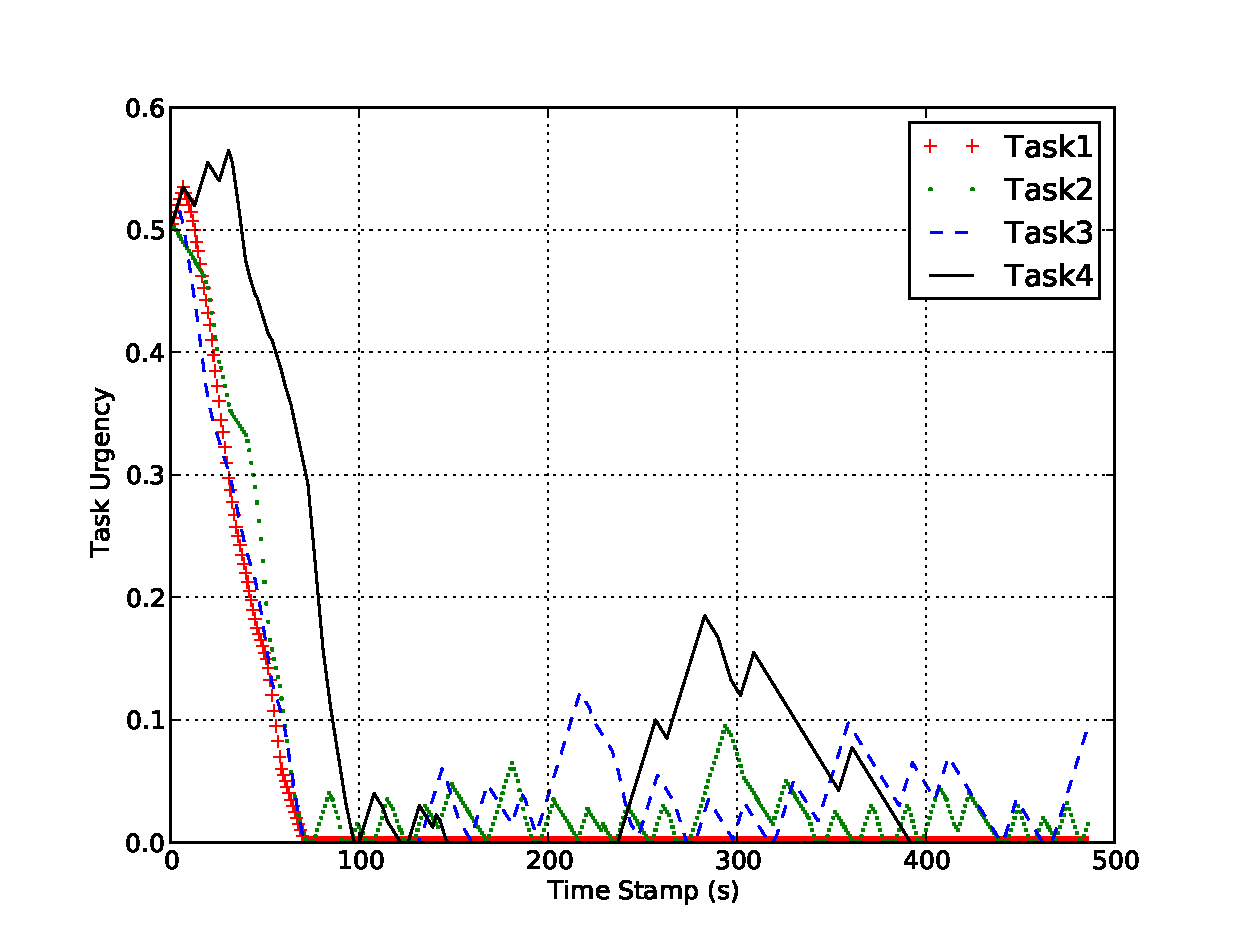
\includegraphics[height=7cm, angle=0]
{images/global/GlobalPlotUrgencyLog-2010Feb18-151600-clear.eps}
%figure caption is below the figure
\caption{\small Task urgencies observed at TaskServer}
\label{fig:raw-urgencies} % Give a unique label
%\end{minipage}
%\hspace{0.5cm}
%\begin{minipage}[t]{0.5\linewidth}
\centering
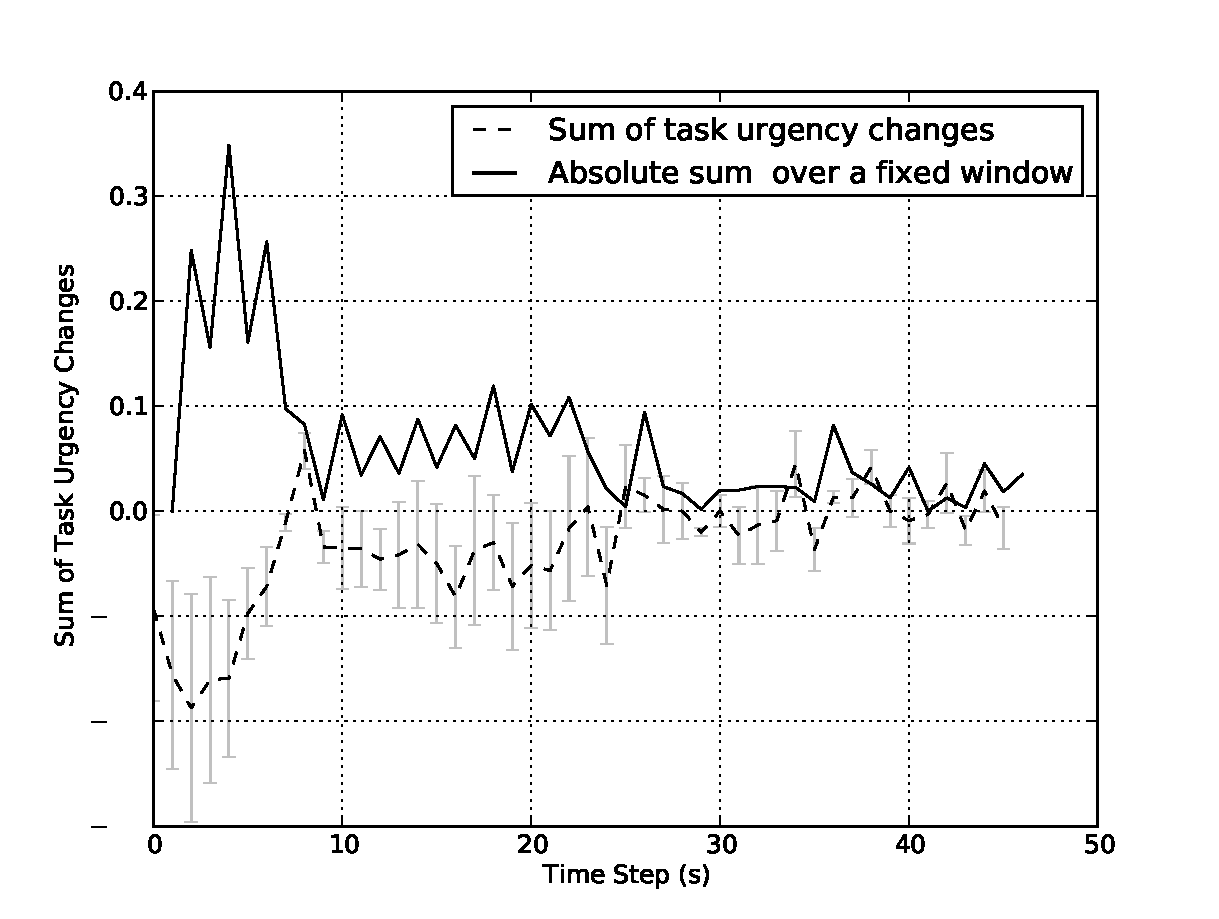
\includegraphics[height=7cm, angle=0]{images/global/TaskUrgencyConvergence-step2-th-p1.eps}
\caption{\small Convergence of task urgencies}
\label{fig:urgency-convergence} % Give a unique label
%\end{minipage}
\end{figure}
%%
%%% Sensitization and Translation %%%
\begin{figure}
\begin{minipage}[t]{0.5\linewidth}
\centering
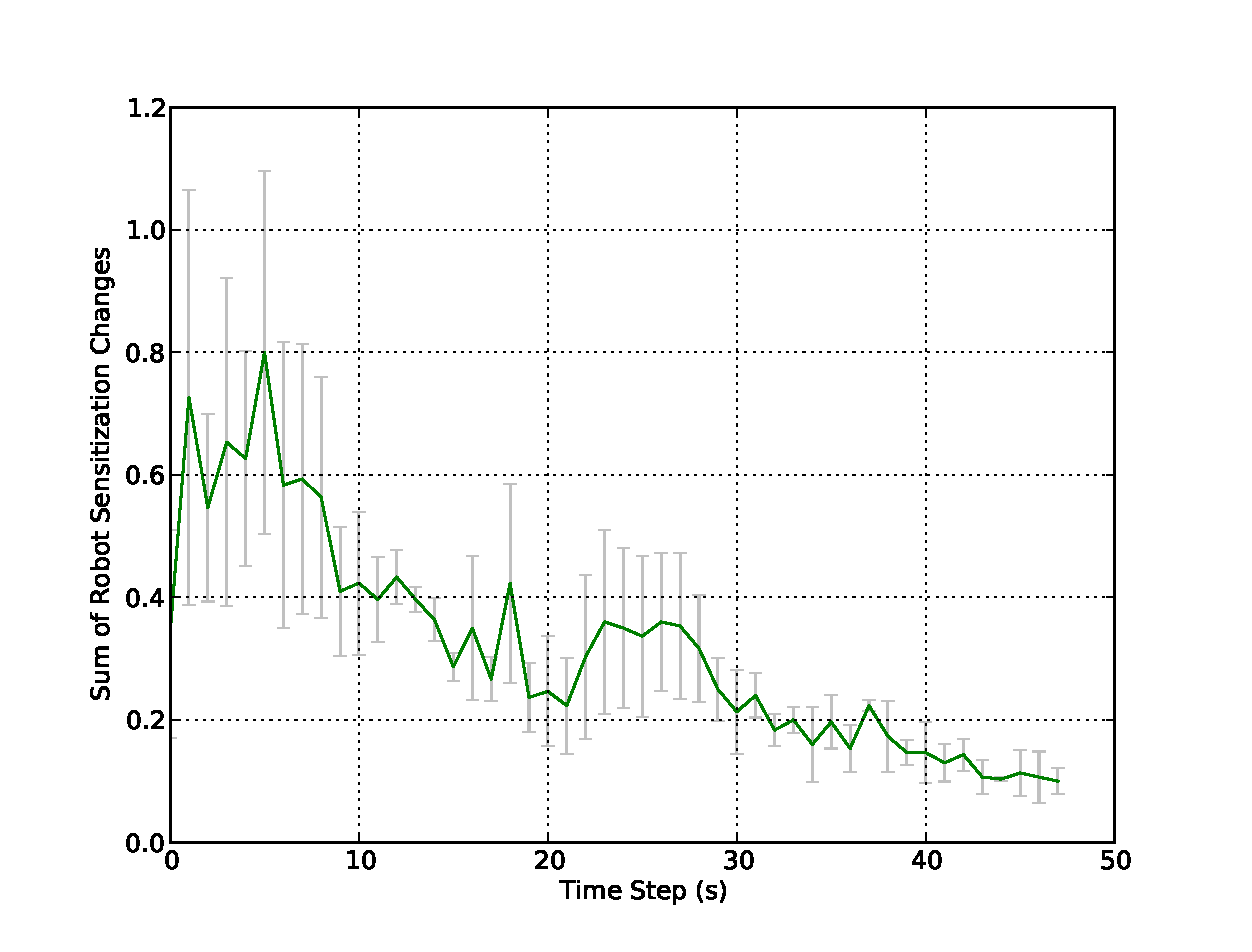
\includegraphics[height=5cm, angle=0]
{images/global/RobotSensitizationStat-Total-50steps.eps}
%figure caption is below the figure
\caption{\small Changes in sensitizations of all robots}
\label{fig:sensitization-stat} % Give a unique label
\end{minipage}
\hspace{0.5cm}
\begin{minipage}[t]{0.5\linewidth}
\centering
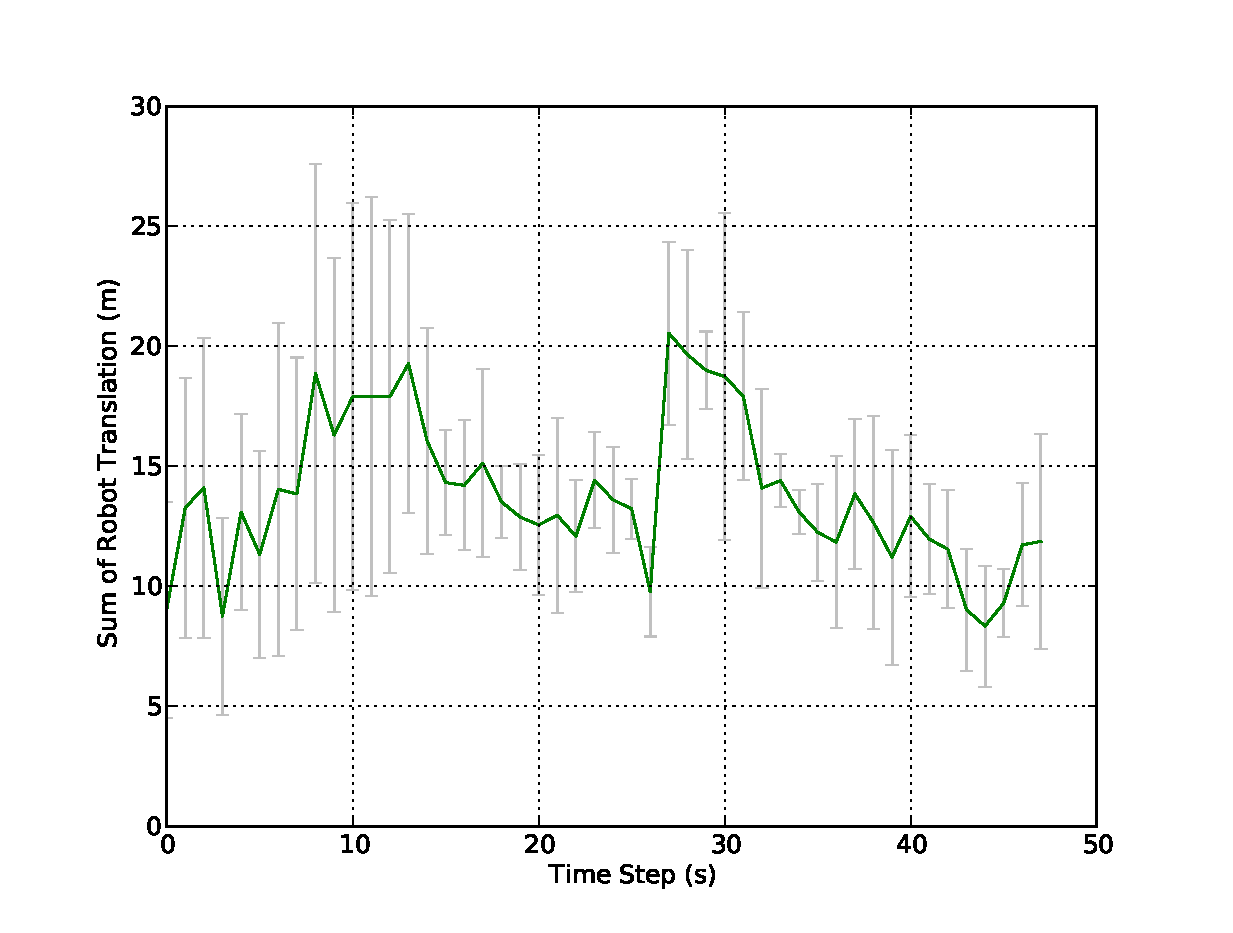
\includegraphics[height=5cm, angle=0]{images/global/DeltaTranslationStat.eps}
\caption{\small Sum of translations of all robots }
\label{fig:translation-stat} % Give a unique label
\end{minipage}
\end{figure}
%%
We have aggregated the changes in translation motion of all robots over time. Let $u_{i,q}$ and $u_{i,q+1}$ be the translations of a robot $i$ in two consecutive steps. If the difference between these two translations be $\delta u_{i}$, we can find the sum of changes of translations of all robots in $(q+1)^{th}$ step using the following equation.
\begin{equation}
\small 
\Delta U_{q+1} = \sum_{i=1}^{N} \delta u_{i, q+1} 
\label{eqn:Delta-Tr}
\end{equation}
This is plotted in Fig. \ref{fig:translation-stat}. Translation is calculated in pixel from the reported pose information by SwisTrack. In this plot we can see that robot translations also vary over varying task requirements of tasks. But it fails to show a consistence behaviour like previous plots.\\
%%% Communication load %%%
\begin{figure}
%\begin{minipage}[t]{0.5\linewidth}
\centering
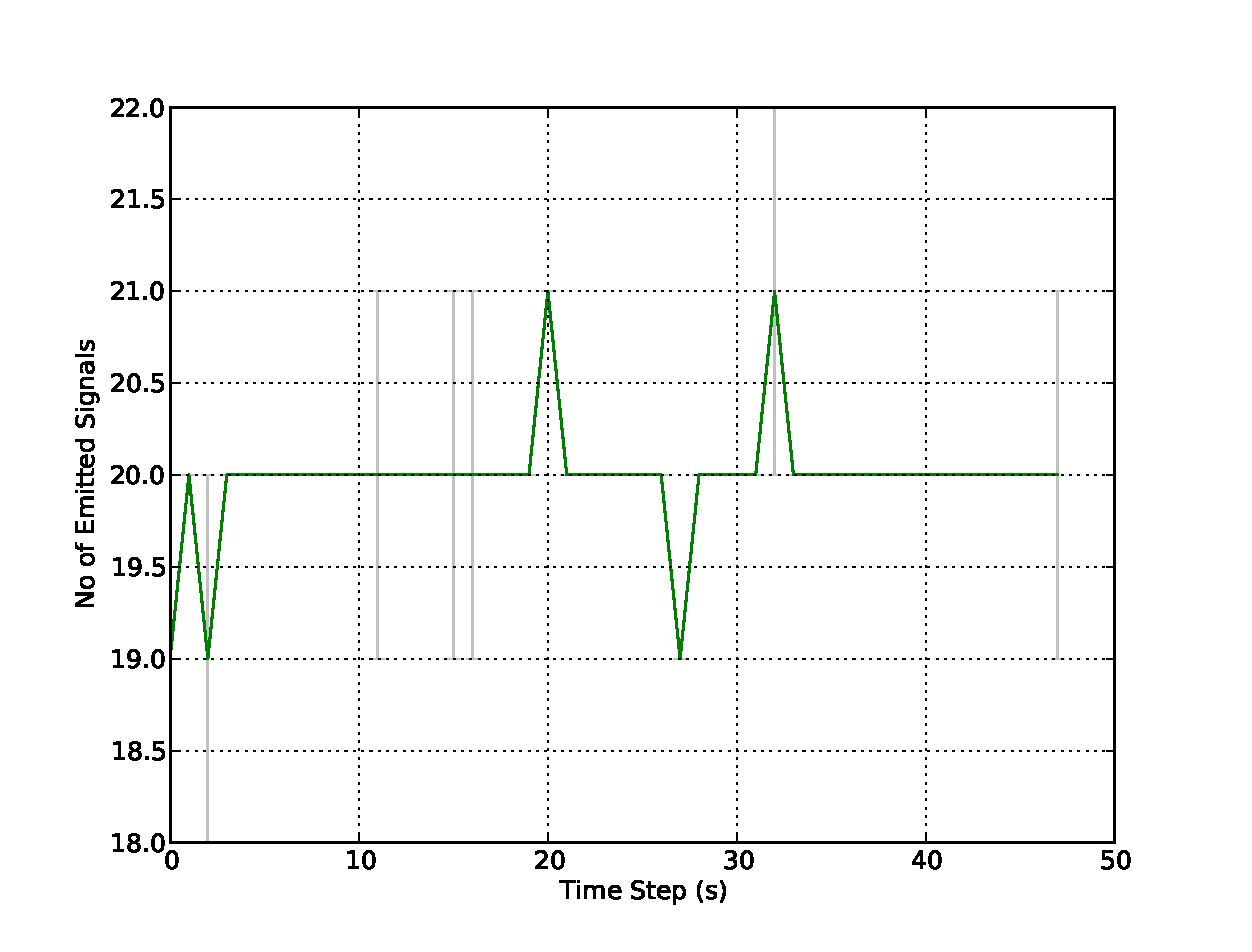
\includegraphics[height=5cm, angle=0]
{images/global/Global-SignalingFreqStat.eps}
%figure caption is below the figure
\caption{\small Task server's frequency of task information signalling}
\label{fig:signal-frequency-stat} % Give a unique label
%\end{minipage}
\end{figure}
Fig. \ref{fig:signal-frequency-stat} presents the frequency of signalling task information by TaskServer. Since the duration of each time step is 50s long and TaskServer emits signal in every 2.5s, there should be 20 signals in each step. The insignificant variation in frequency shows us the stable behaviour of D-Bus daemon over time.
\begin{figure}
\begin{minipage}[t]{0.5\linewidth}
\centering
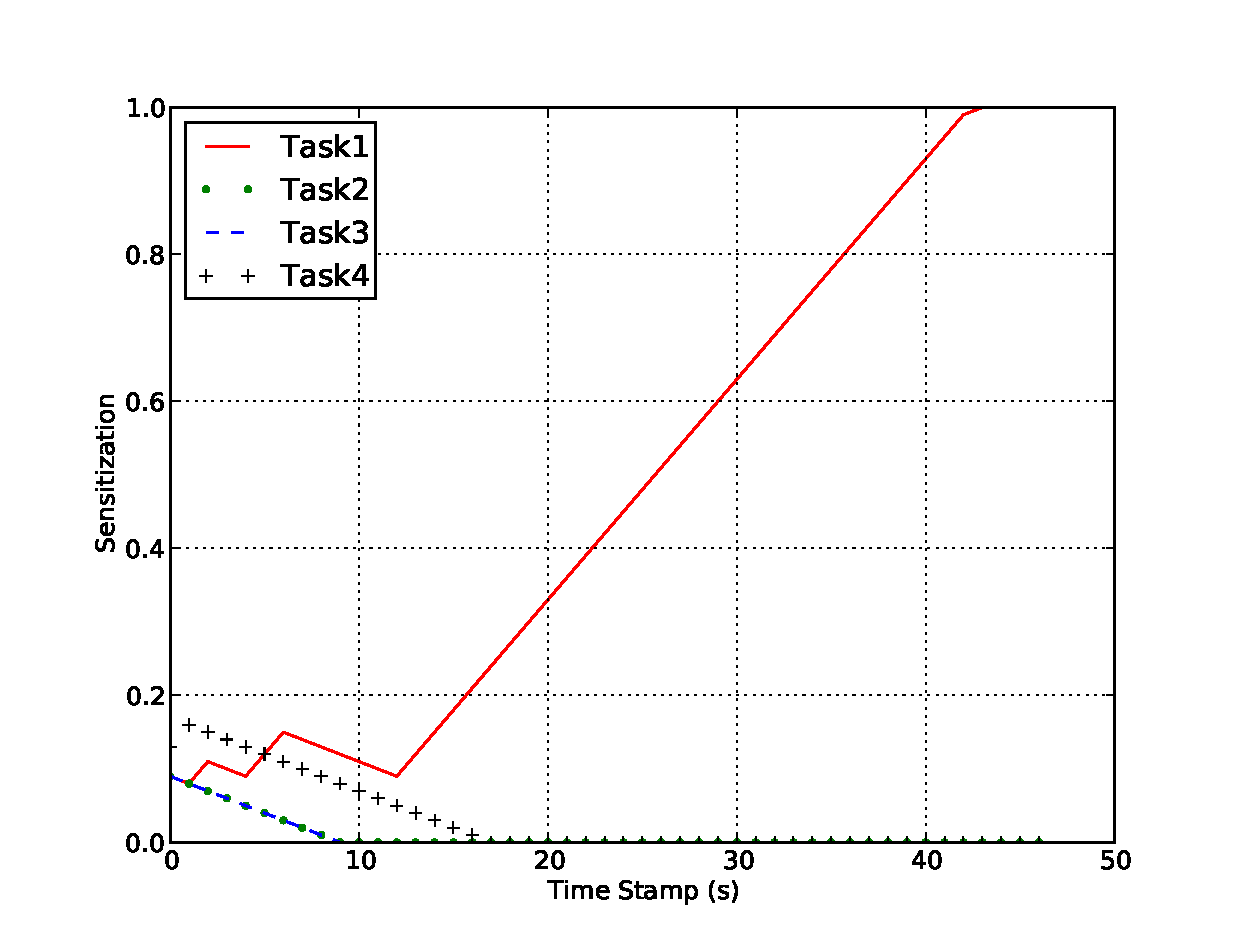
\includegraphics[height=5cm, angle=0]{images/global/PlotRobot9-Sensitizations-2010Feb18-121037.eps}
\caption{\small Task specialization of Robot9}
\label{fig:single-robot-sensitizations} % Give a unique label
\end{minipage} 
%%%
\begin{minipage}[t]{0.5\linewidth}
\centering
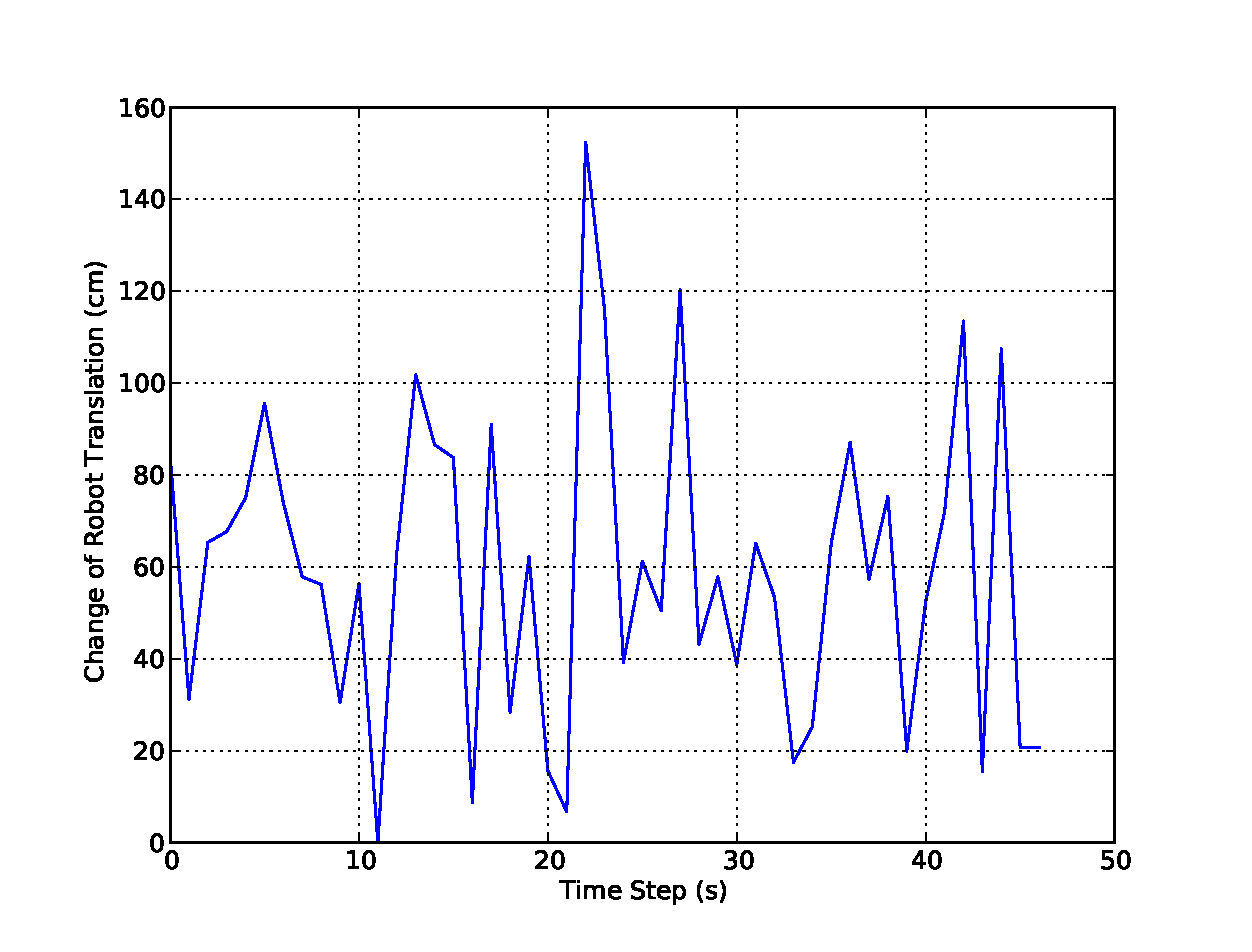
\includegraphics[height=5cm, angle=0]{images/global/DeltaRobot9-PoseAtTS-2010Feb18-121037.eps}
\caption{\small Changes in translation of Robot9}
\label{fig:single-robot-translation} % Give a unique label
\end{minipage}
\end{figure}
As an example of task specialization of a robot we plotted sensitization of Robot9 in Fig. \ref{fig:single-robot-sensitizations}. It shows that this robot has specialized in Task1. The continuous learning happens from step 12 to step 42 where it has learned this task completely and forget rest of the tasks. This is common in all robots with varying level of sensitizations. Hence we get the linear decrease of $\Delta K$ in Fig. \ref{fig:sensitization-stat}. However, the changes in motion of this robot plotted in Fig. \ref{fig:single-robot-translation} is not stable due to the fact that robots frequently avoid dynamic obstacles and select random walks to do so.
%%%%%%%%%%%%%%%%%%%%%%%%%%%%%%%%%%%%%%%%%%%%%%%%%%%%%%%%%%%%%%%%
\section{Conclusion and Future works}
\label{sec:conc}
In this paper we have validated an inter-disciplinary generic model of self-regulated division of labour by incorporating it in our physical robotic social system. A centralized communication system has been instantiated to realize this model. We have evaluated various aspects of this model such as ability to meet dynamic task demands, individual task specializations, communication loads and flexibility in concurrent task completions over time. A set of metrics has been proposed to observe the convergence of division of labour in this system. From our experimental evidences, it is clear that such a system can meet the requirements of dynamic division of labour of a multi-robot system by the virtue of its self-regulatory behaviours. One drawback of our current implementation is that this system maintains a constant communication load on the system even the task requirements change. Certainly, this will prevent us from scaling up the system. Therefore, we would like to extend our work by validating this model with different number of tasks and robots using a local peer-to-peer communication strategy. Our aim is to implement this model in a multi-robot system having up to 40 E-puck robots that works in a relatively larger area.
%\begin{acknowledgements}
%If you'd like to thank anyone, place your comments here
%and remove the percent signs.
%\end{acknowledgements}
% BibTeX users please use one of
%\bibliographystyle{spbasic} % basic style, author-year citations
%\bibliographystyle{spmpsci} % mathematics and physical sciences
%\bibliographystyle{spphys} % APS-like style for physics
%\bibdata{bib-intro}
%\bibliography{bib-intro} % name your BibTeX data base
% Non-BibTeX users please use
\begin{thebibliography}{}
% and use \bibitem to create references. Consult the Instructions
% for authors for reference list style.
\bibitem{Camazine+2001}
Camazine, S., Franks, N., Sneyd, J., Bonabeau, E., Deneubourg, J. and Theraulaz, G.: Self-organization in biological systems.
Princeton University Press, Princeton, N.J (2001)

\bibitem{Bonabeau+1999}
Bonabeau, E., Dorigo, M. and Theraulaz, G.:
Swarm intelligence: from natural to artificial systems.
Oxford University Press (1999)

\bibitem{Gerkey+2004}
Gerkey, B. P. and Mataric M. J.:
A Formal Analysis and Taxonomy of Task Allocation in Multi-Robot Systems.
The International Journal of Robotics Research, 23  (2004)

\bibitem{Parker2008}
Parker, L. E.:
Distributed Intelligence: Overview of the Field and its Application in Multi-Robot Systems.
Journal of Physical Agents,  2, 5-14 (2008)

\bibitem{Lerman+2006}
Lerman, K., Jones, C., Galstyan, A. and Mataric, M. J.:
Analysis of Dynamic Task Allocation in Multi-Robot Systems. 
The International Journal of Robotics Research, 25, 225  (2006)

\bibitem{Shen+2001}
Shen, W., Hao, Q., Yoon, H. and Norrie, D.:
Applications of agent-based systems in intelligent manufacturing: An updated review. Advanced Engineering Informatics, 20, 415-431, Elsevier (2006)

\bibitem{Dias+2006}
Dias, M. B., Zlot, R. M., Kalra, N. and Stentz, A.:
Market-based multirobot coordination: A survey and analysis. 
Proceedings of the IEEE, 94, 1257-1270,  IEEE  (2006)

\bibitem{Liu+2007} 
Liu, W., Winfield, A. F. T., Sa, J., Chen, J. and Dou, L.:
Towards Energy Optimization: Emergent Task Allocation in a Swarm of Foraging Robots. Adaptive Behavior, 94, 1257-1270 (2007)

\bibitem{Sayer+1992}
Sayer, A. and Walker, R.: 
The new social economy : reworking the division of labor.
Blackwell (1992)

\bibitem{Beer1981}
Beer, S.: 
Brain of the firm.
J. Wiley New York (1981)

\bibitem{Kogut2000}
Kogut, B.: 
The network as knowledge: generative rules and the emergence of structure. 
Strategic Management Journal, 21, 405-425 (2000)
\bibitem{Swarm}
% Format for Journal Reference
Sahin E. and Winfield A.: 
Special issue on swarm robotics.
Swarm Intelligence, 2, 69-72 (2008)
% Format for books
\bibitem{Elsa}
Arcaute, E.; Christensen, K.; Sendova-Franks, A.; Dahl, T.; Espinosa, A. and Jensen, H. J. : 
Division of labour in ant colonies in terms of attractive fields. 
Ecological Complexity, Elsevier (2008)
% etc
\bibitem{SwisTrack}
Lochmatter T., Roduit P., Cianci C., Correll N., Jacot J., and Martinoli A.: 
SwisTrack - A Flexible Open Source Tracking Software for Multi-Agent Systems. 
In Proceedings of the IEEE/RSJ 2008 International Conference on Intelligent Robots and Systems (IROS 2008), 4004-4010, IEEE (2008)
\bibitem{Epuck}
Mondada, F., Bonani, M., Raemy, X., Pugh, J., Cianci, C., Klaptocz, A., Magnenat, S., Zufferey, J.-C., Floreano, D. and Martinoli, A.:
The e-puck, a Robot Designed for Education in Engineering. 
Proceedings of the 9th Conference on Autonomous Robot Systems and Competitions, 1(1) 59-65 (2009) 
\bibitem{DBus}
http://www.freedesktop.org/wiki/Software/dbus
\bibitem{Multiprocessing}
http://docs.python.org/library/multiprocessing.html
\bibitem{bustle}
http://willthompson.co.uk/bustle/
\end{thebibliography}
%
\end{document}